% Appendix A

\chapter{FAST (Fatigue, Aerodynamics, Structures, and Turbulence) } % Main appendix title

\label{AppendixA} % For referencing this appendix elsewhere, use \ref{AppendixA}

\lhead{Appendix A. \emph{Sample FAST Simulation Input Files}} % Change X to a consecutive letter; this is for the header on each page - perhaps a shortened title

FAST is a medium fidelity aeroelastic wind turbine modeling tool developed by NREL and Oregon State University. This dissertation uses FAST v7, which is documented in \cite{jonkman2005,jonkman2013a,jonkman2013}. FAST models turbine structural dynamics as a combination of modal dynamics and multibody dynamics. FAST models aerodynamic loading on the turbine using blade-element/momentum (BEM) theory. FAST is widely used in the wind industry and has been independently validated and verified[14].

FAST models turbine structural dynamics as a combination of modal dynamics and multibody dynamics. As shown in Figure \ref{figA-1}, a FAST model of a horizontal axis 3 blade turbine has 24 structural degrees of freedom. thirteen of those degrees of freedom are associated with bending modes of the blades and tower, while the other eleven are associated with rigid body motion of the drivetrain, nacelle, furl, and platform. FAST allows users to disable degrees of freedom that are not needed. For example, in this dissertation the furl and platform degrees of freedom were not used because the NREL 5-MW turbine does not have furling hinges and the turbine was assumed to be on solid ground, not a floating platform. 

\begin{figure}[ht]
	\centering
		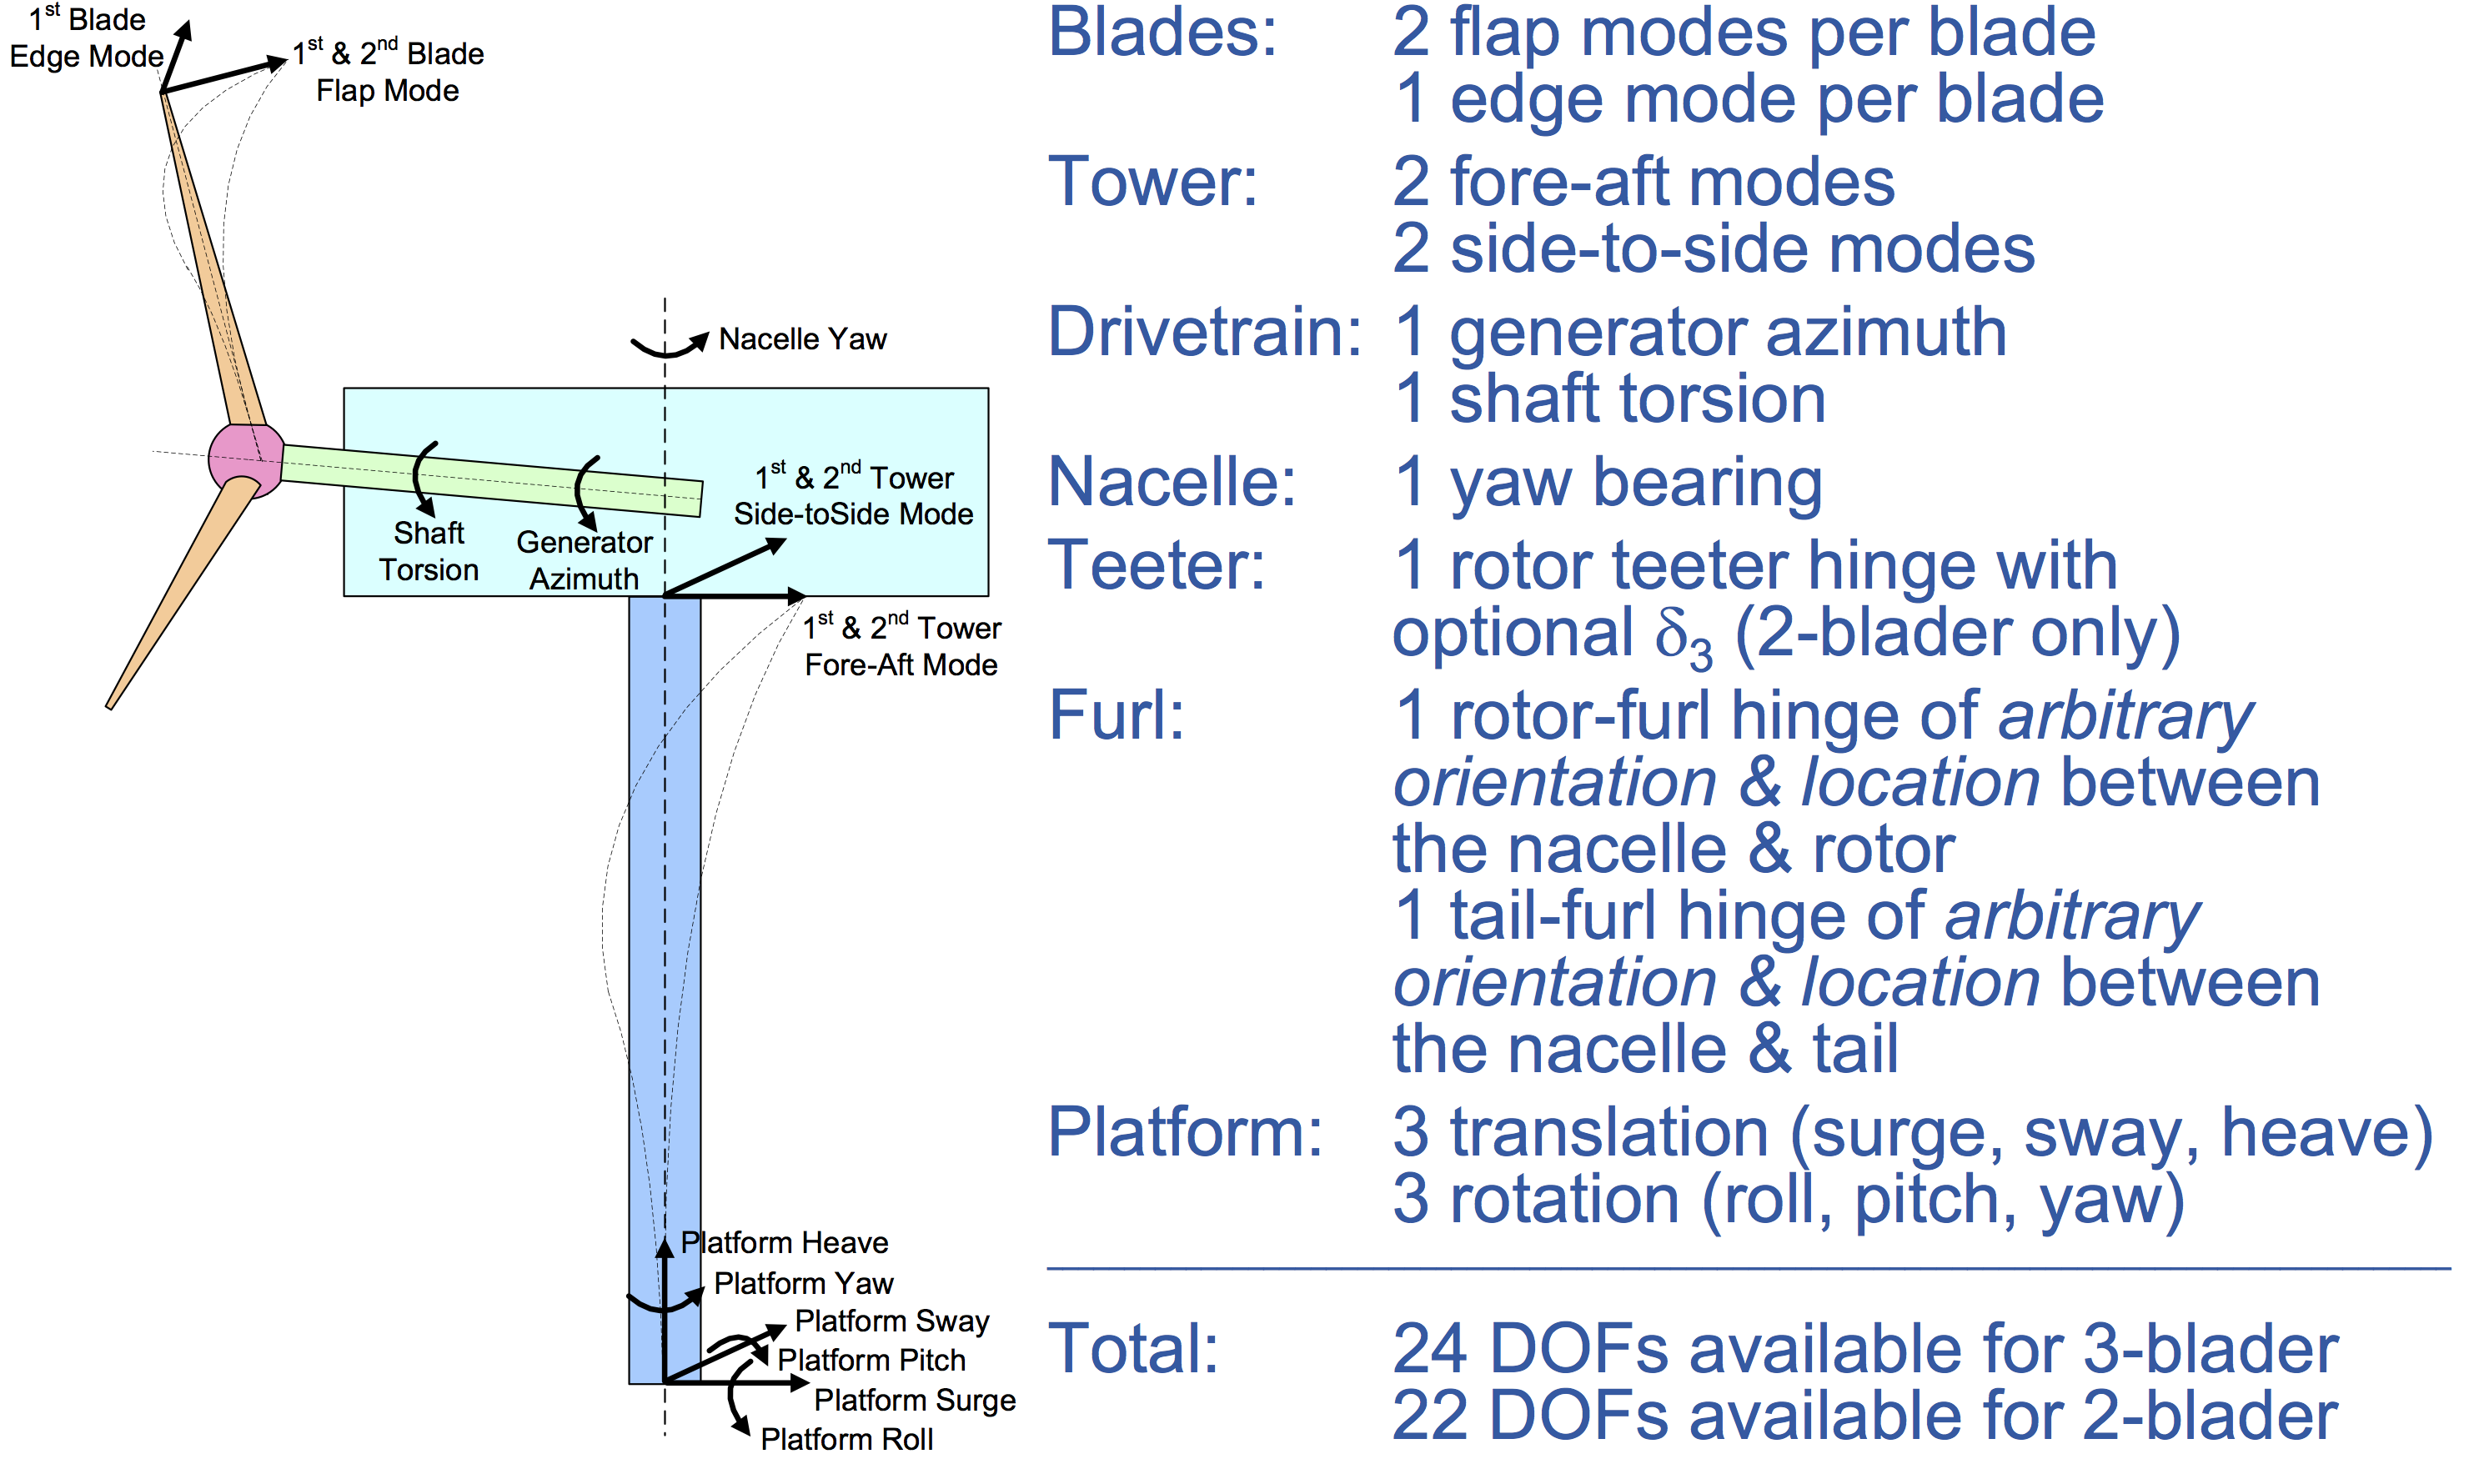
\includegraphics[width=\linewidth]{Figures/AppendixAFigures/figA-1.png}
	\caption{structural degrees of freedom of a FAST turbine model.\cite{jonkman2013}}
	\label{figA-1}
\end{figure}


The turbine blades and tower are modeled as Bernoulli-Euler beams under bending. The first two bending modes are modeled for blade flapwise bending, tower fore-aft bending, and tower side-to-side bending. The first bending mode is modeled for blade edgewise bending. No higher order bending modes, or torsional twisting modes are modeled. Figure \ref{figA-4} illustrates typical first and second bending mode shapes for a turbine tower.

\begin{figure}[ht]
	\centering
		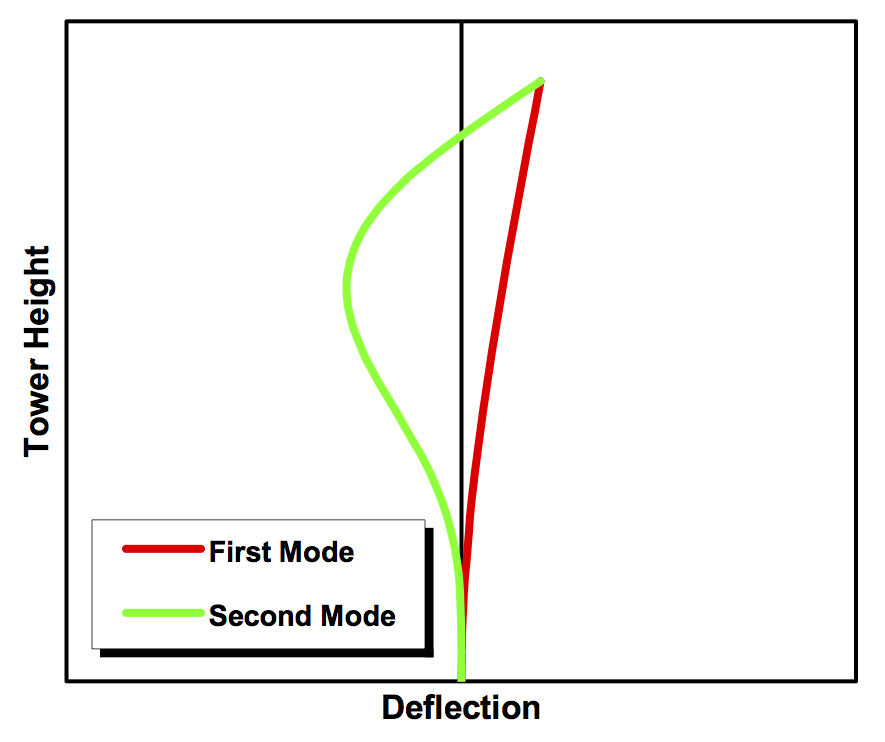
\includegraphics[width=.5\linewidth]{Figures/AppendixAFigures/figA-4.png}
	\caption{First and second tower bending mode shapes.\cite{jonkman2005}}
	\label{figA-4}
\end{figure}

The nonlinear equations of motion are obtained using Kane's method. In Kane's method, the motion of a dynamic system is described by a set of generalized coordinates and generalized speeds. Rigid body innertias and forces external to the system are described by a set of generalized forces. Kane's method does not require knowledge of internal forces that bodies in the dynamic system exert on each other. Figure \ref{figA-2} shows a double pendulum and one set of generalized coordinates that could be used to describe the system, $q_1$ and $q_2$. Generalized coordinates are not unique. Another set of coordinates could be chosen as long as they fully define the configuration of the system. For this example the generalized speeds would be $dot{q}_1$ and $dot{q}_2$, the first derivatives of the generalized coordinates. This example would have generalized forces associated with the gravitational force on the pendulum mass and the innertia of the pendulum mass. Internal forces, such as the forces exerted through the hinges, would not factor into the calculations. Kane's method is highly systematic and is especially well suited for complicated dynamic systems with many interconnected bodies. Detailed instructions for obtaining equations of motion through Kane's method can be found in \cite{kane1985} and \cite{roithmayr2016}.

\begin{figure}[ht]
	\centering
		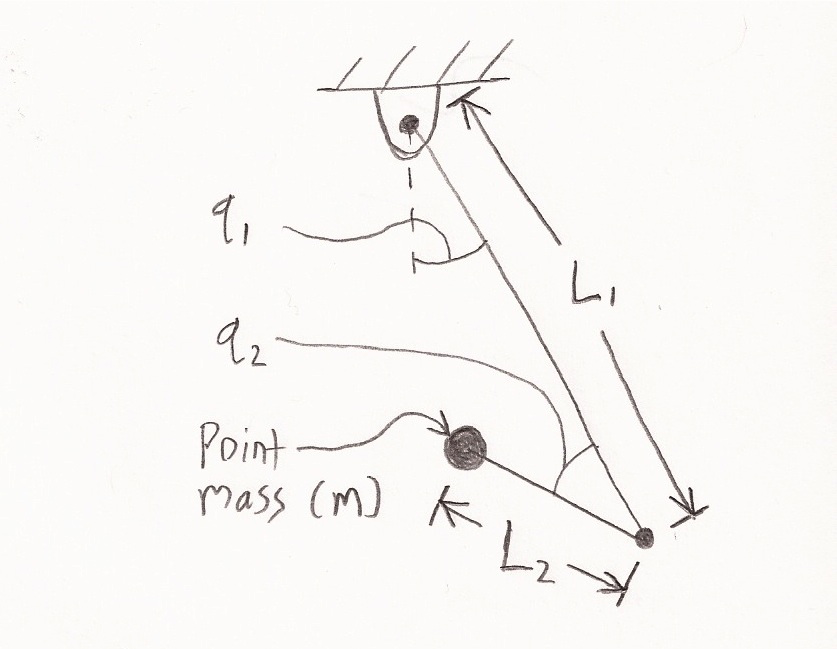
\includegraphics[width=.5\linewidth]{Figures/AppendixAFigures/figA-2.png}
	\caption{A double pendulum and a set of generalized coordinates that could be used to derive the equations of motion via Kane's method.}
	\label{figA-2}
\end{figure}


FAST models aerodynamics using blade-element/momentum theory (BEM). Turbine rotor aerodynamics are complex and three dimensional. BEM approximates this complex flow using a large number of simpler (and computationally inexpensive) 2-D airflow calculations. In BEM theory, turbine blades are treated as a collection of discrete 2-D airfoil segments that move in space as the turbines blades rotate (Figure \ref{figA-3}). The aerodynamic forces on each airfoil segment are determined from the local air flow field, as well as the motion, orientation, and 2-D aerodynamic properties of the airfoil. The aerodynamic forces on the rotor are determined by summing the forces on all of the blade segments and applying a series of correction factors to account for 3-D flow effects such as tip vortices, root vortices, and dynamic stall. 

\begin{figure}[ht]
	\centering
		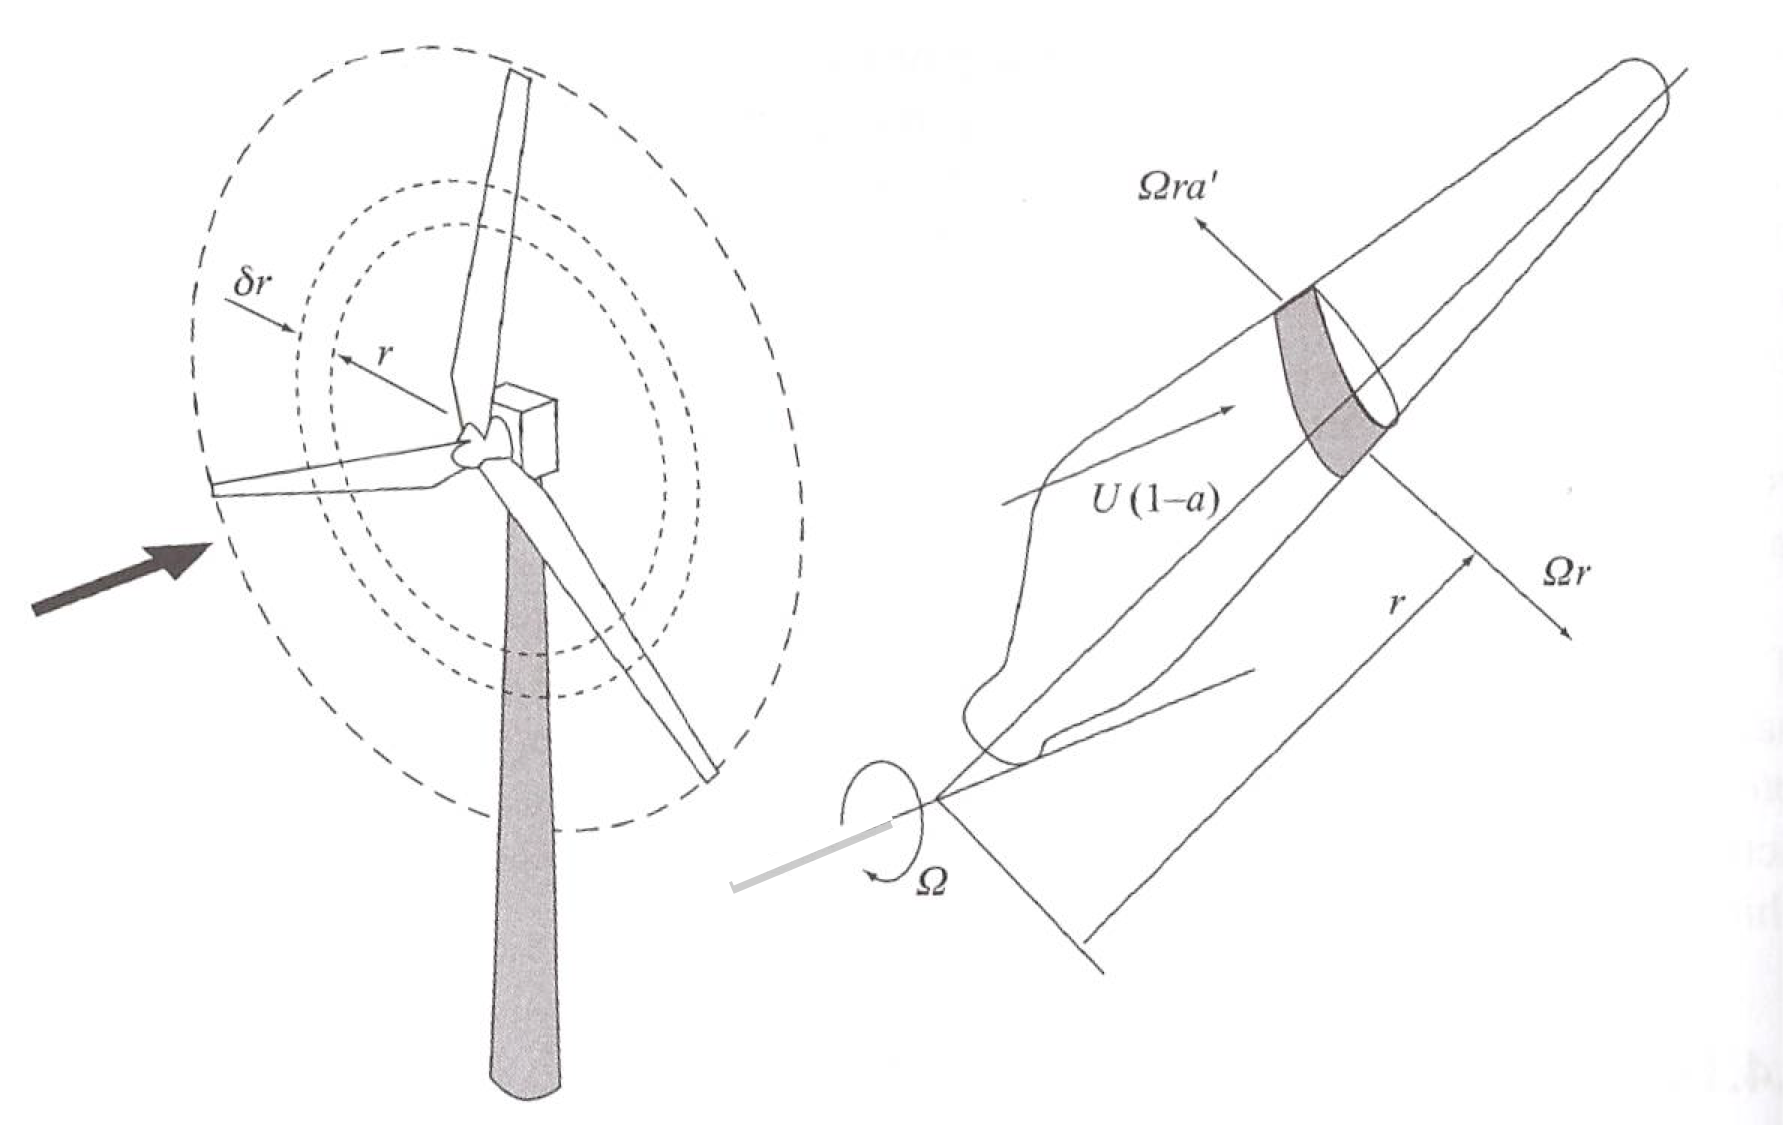
\includegraphics[width=.75\linewidth]{Figures/AppendixAFigures/figA-3.png}
	\caption{BEM models each turbine blade as a collection of spanwise blade segments.\cite{burton2011}}
	\label{figA-3}
\end{figure}

The following pages contain samples of the \textit{primary.fst} and \textit{Aerodyn.ipt} FAST input files. Many FAST simulations were run in this dissertation and some settings varied from one simulation to another, but the parameters shown in these input files illustrate typical settings used in this dissertation. FAST also uses input files to specify the wind flow field, the structural properties of the turbine tower,  and the structural and aerodynamic properties of the turbine blades. Those other input files have not been included here because they are either dictated by the properties of the NREL 5-MW turbine, or they are generated by another simulation tool.

FAST has a variety of options for modeling turbine control. Those options are specified in the \textit{TURBINE CONTROL} section of \textit{primary.fst}. FAST can model turbine yaw, pitch, and variable speed control, as well as a number of control events such as brake deployments, pitch override maneuvers, and yaw override maneuvers. If dynamic control is not desired, a control mode can be completely disabled. For example, the FAST simulations in this dissertation did not require dynamic yaw control so yaw control was disabled in FAST ($YCMode = 0$). A simple variable speed control can be based on the input parameters $VS\_RtGnSp$, $VS\_RtTq$, $VS\_Rgn2K$, and $VS\_SlPc$. However, that method was not used in this dissertation. FAST can also model yaw, pitch, and variable speed control as a set of user defined subroutines or can interface with controllers modeled in Simulink. For FAST simulations in this dissertation, Simulink based controllers were used for pitch and variable speed control. These Simulink based controllers are documented in Appendix \ref{AppendixB}.

In FAST simulations, the wind is defined by an input wind file. FAST accommodates two types of wind file, hub height wind files and full field wind files. Hub height wind files are text files specifying hub height wind speed, wind direction, and wind shear at several moments in time. FAST models wind by interpolating data in the hub height wind file. A full field wind file is a binary file containing two dimensional grids of three component wind speed data. FAST models wind by marching these grids of wind speed data past the turbine at the mean wind speed. This dissertation uses both hub height wind files and full field wind files.

Several tools can be used to generate full field wind files. the Full field wind files used in this dissertation were generated using TurbSim.\cite{jonkman2012} Turbsim uses a statistical model, along with Taylor's frozen turbulence hypothesis to generate full field, turbulent wind files. TurbSim files can capture realistic boundary layer effects that are based on experimental data gathered at a variety of wind sites. Many of the full field wind files used in this dissertation use the Great Planes Low Level Jet (GPLLJ) spectral model, which is based on experimental data gathered in southeastern Colorado.


\pagebreak
\section{primary.fst} \label{sectionA-1}

\noindent
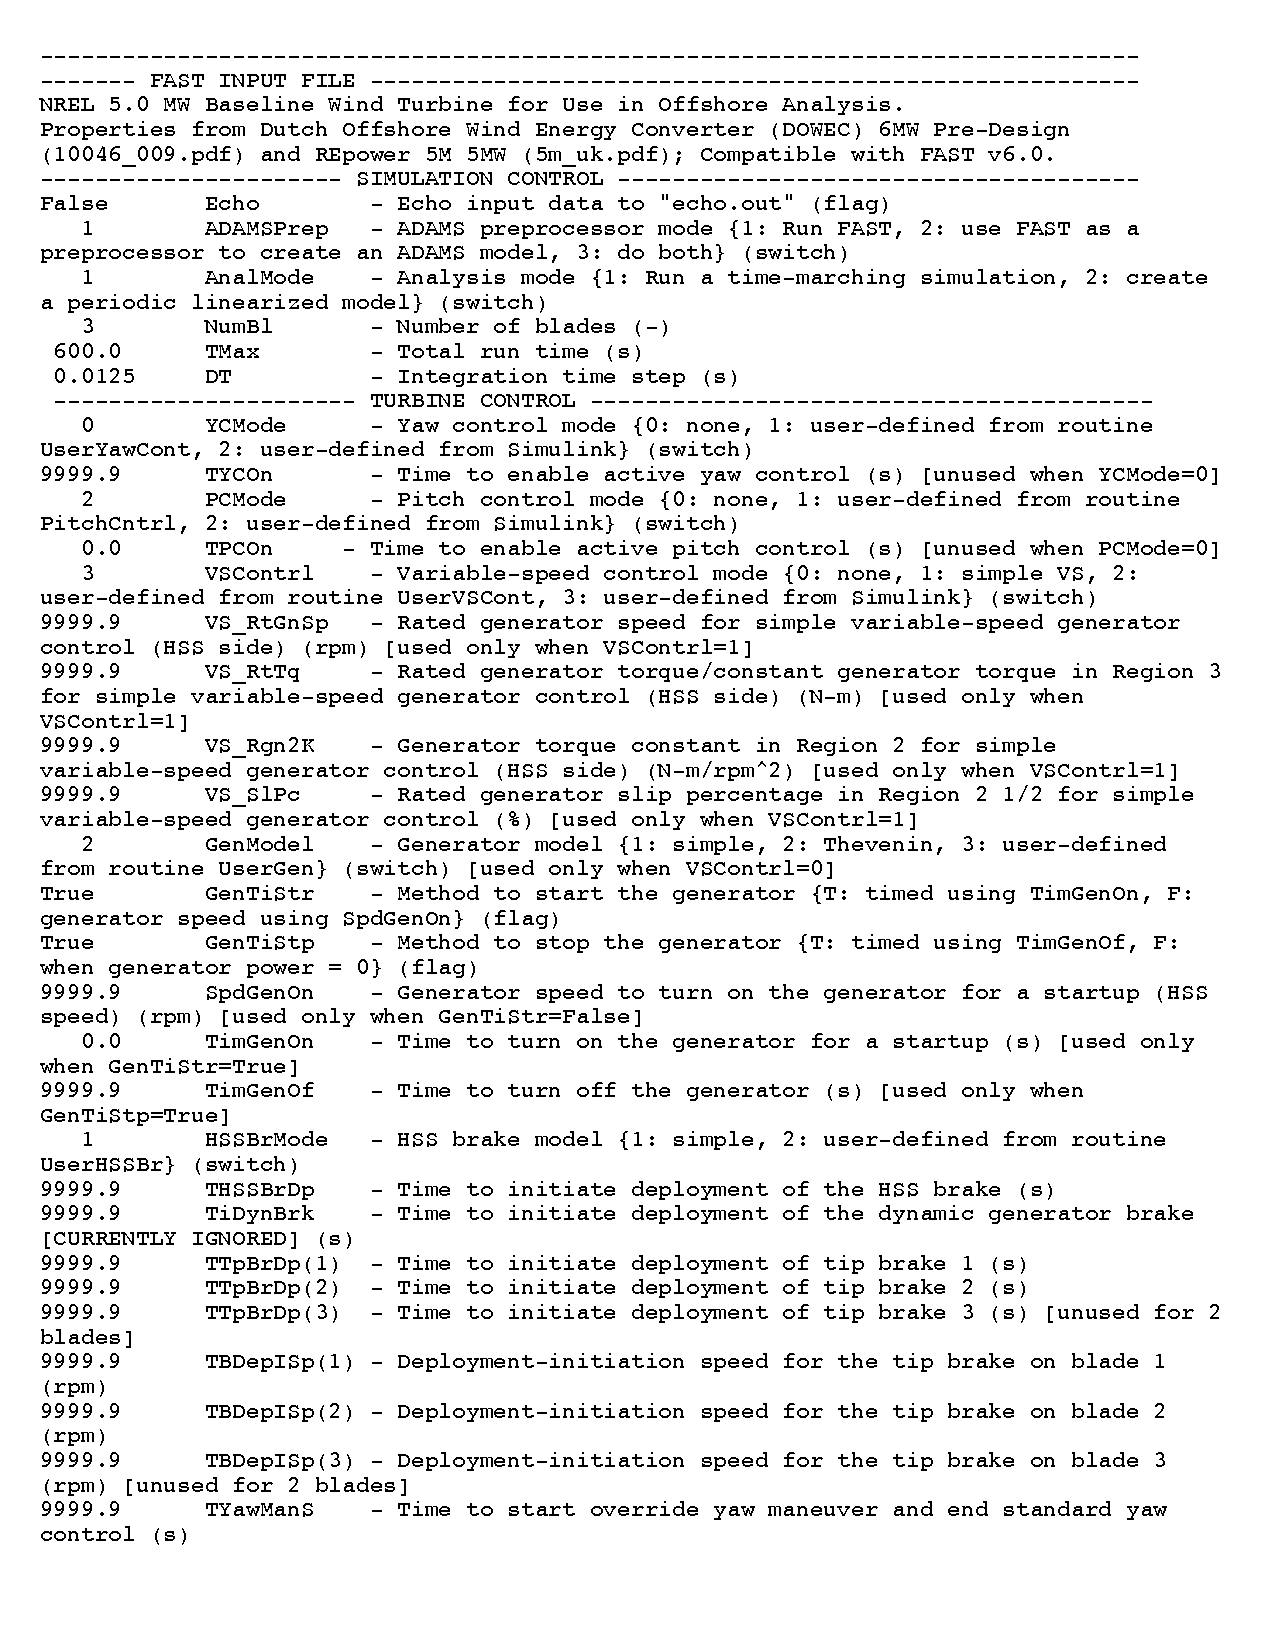
\includegraphics[width=\linewidth]{Figures/AppendixAFigures/primaryP1.pdf}		

\noindent
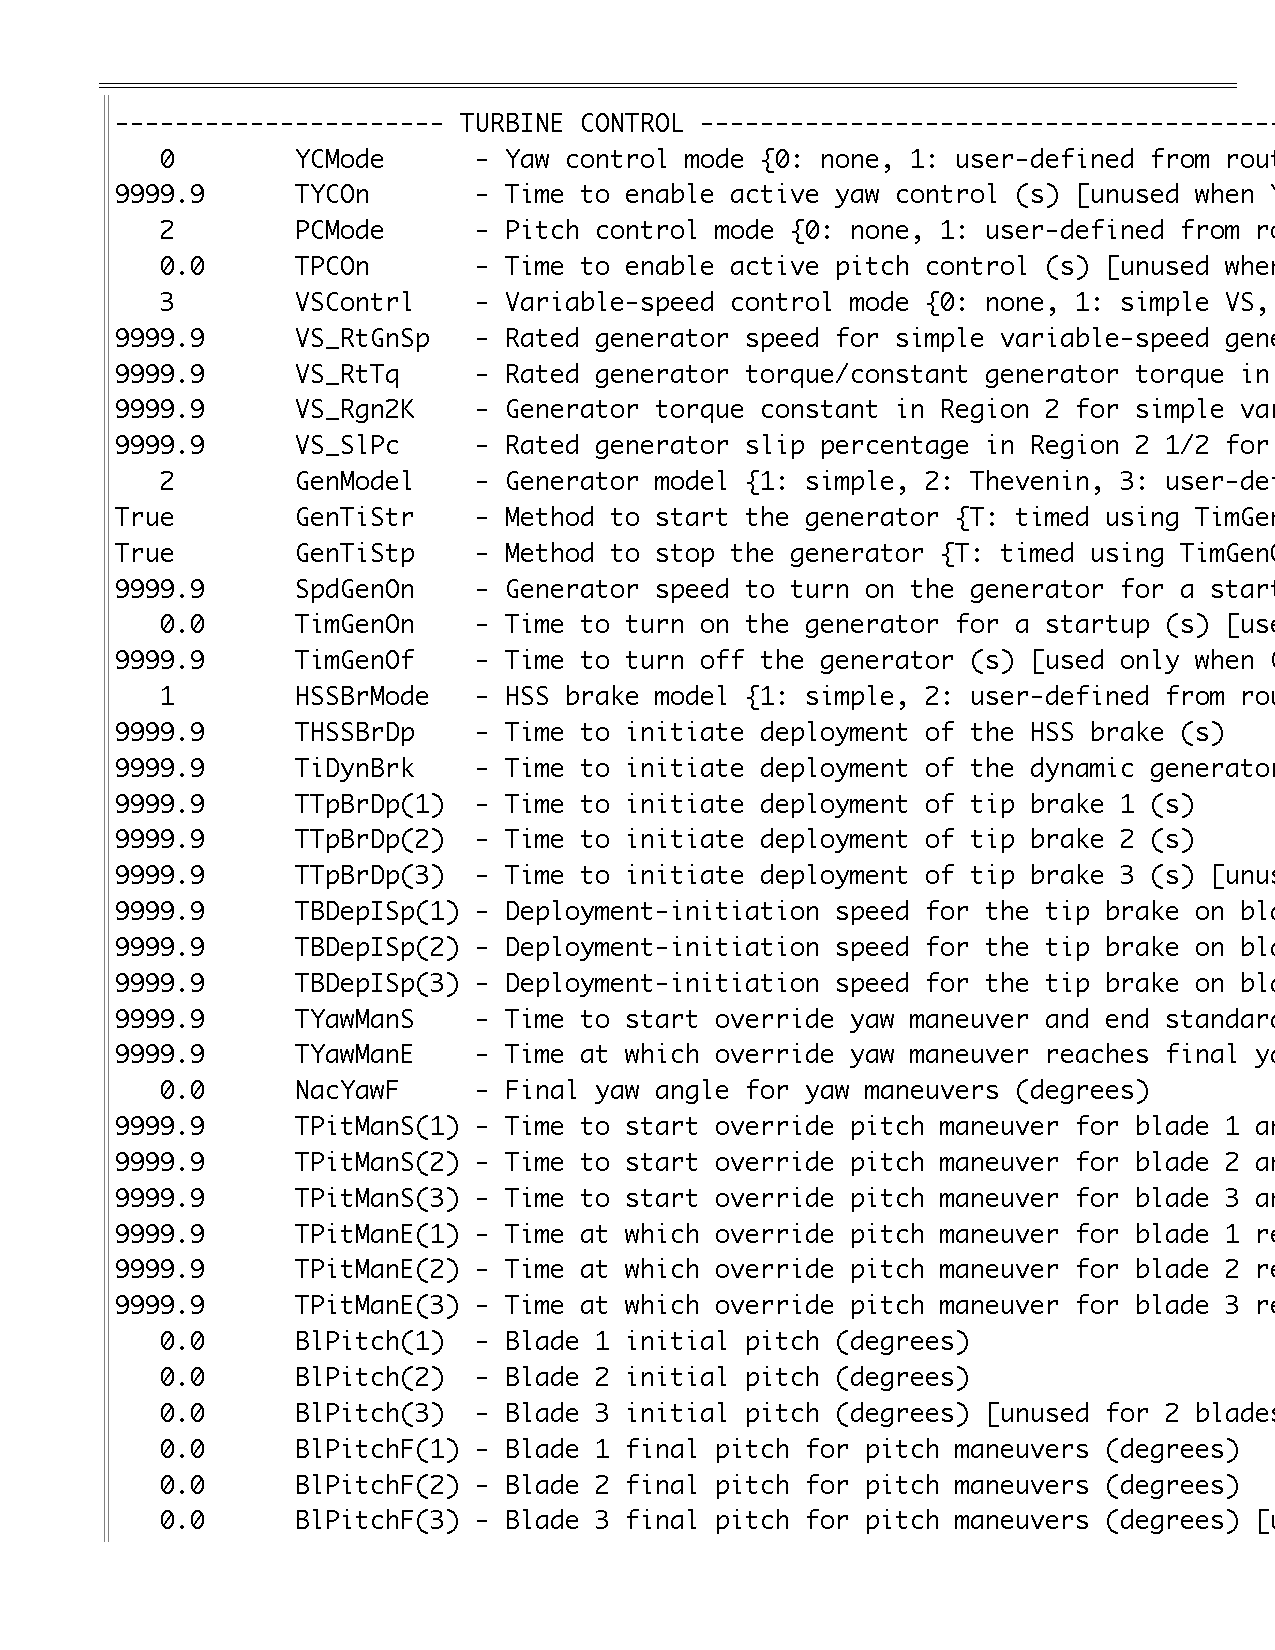
\includegraphics[width=\linewidth]{Figures/AppendixAFigures/primaryP2.pdf}

\noindent
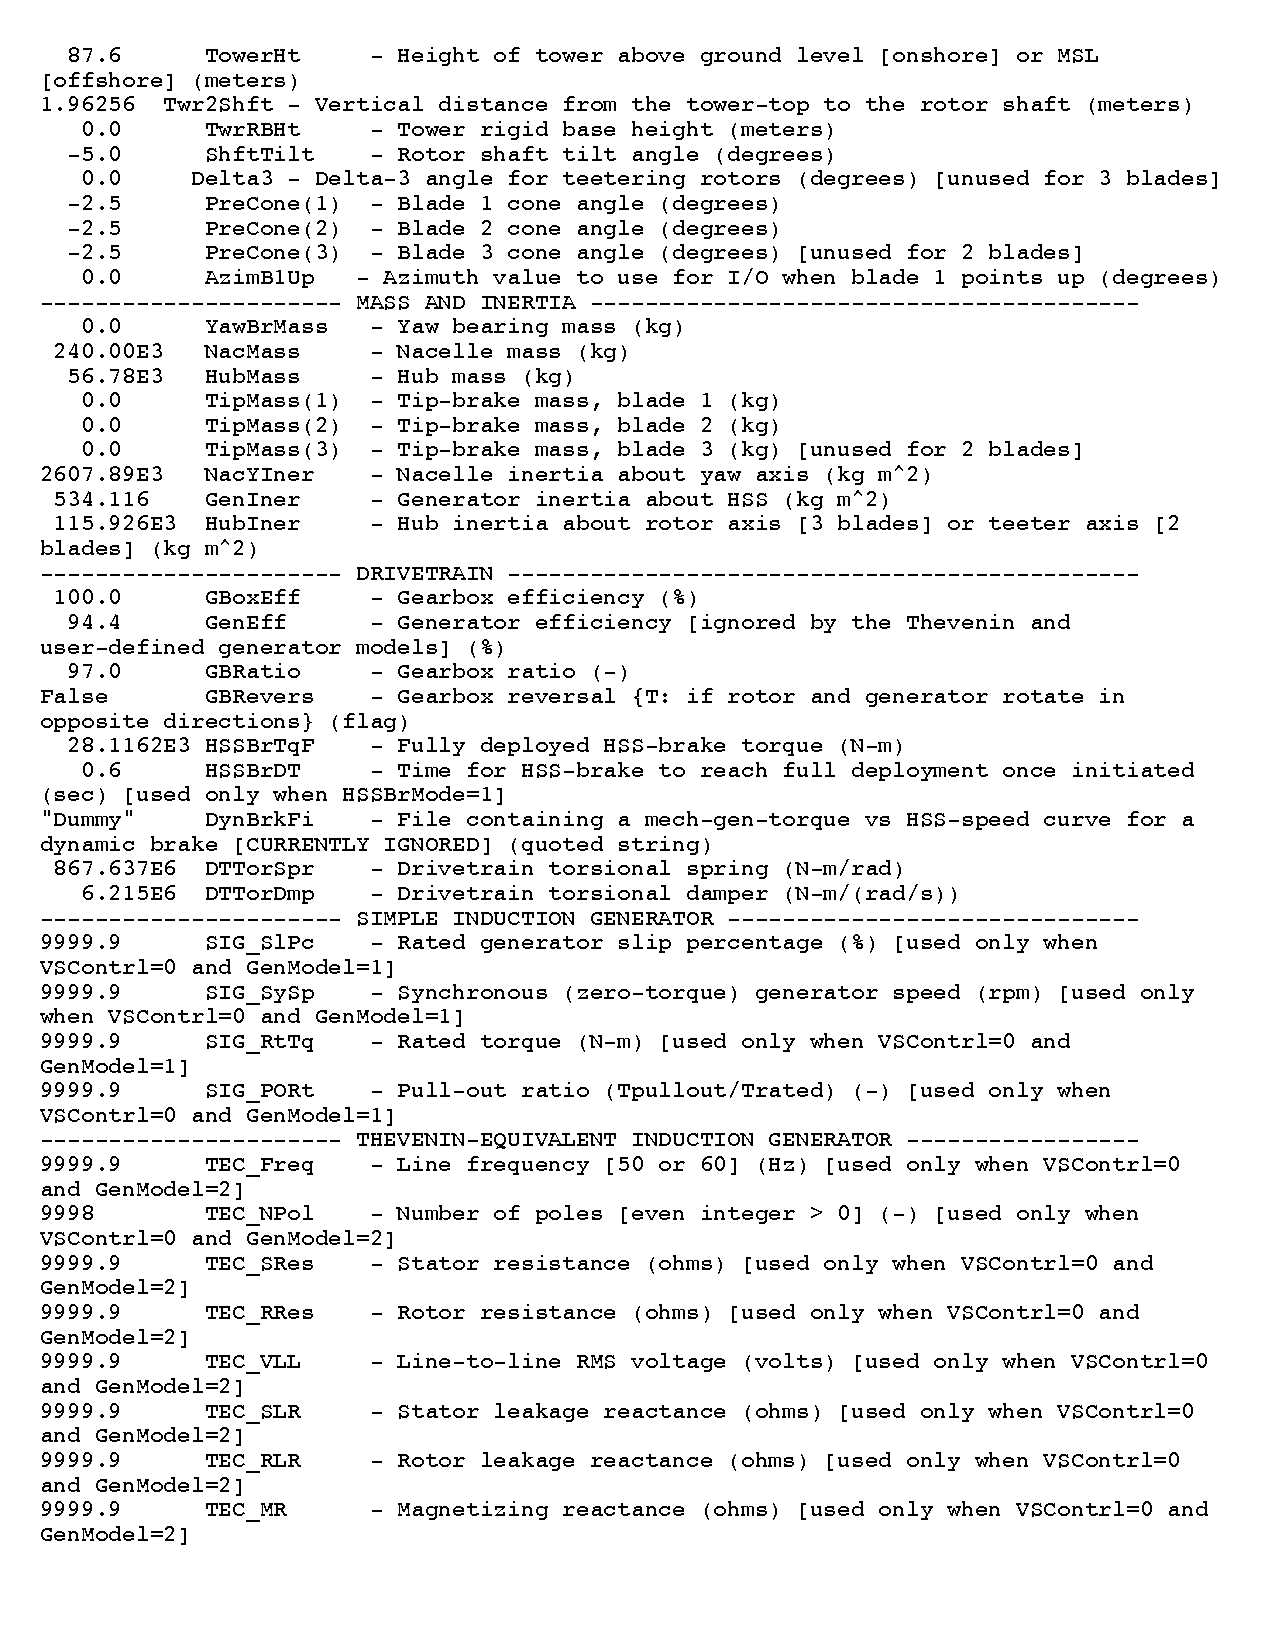
\includegraphics[width=\linewidth]{Figures/AppendixAFigures/primaryP3.pdf}	

\noindent
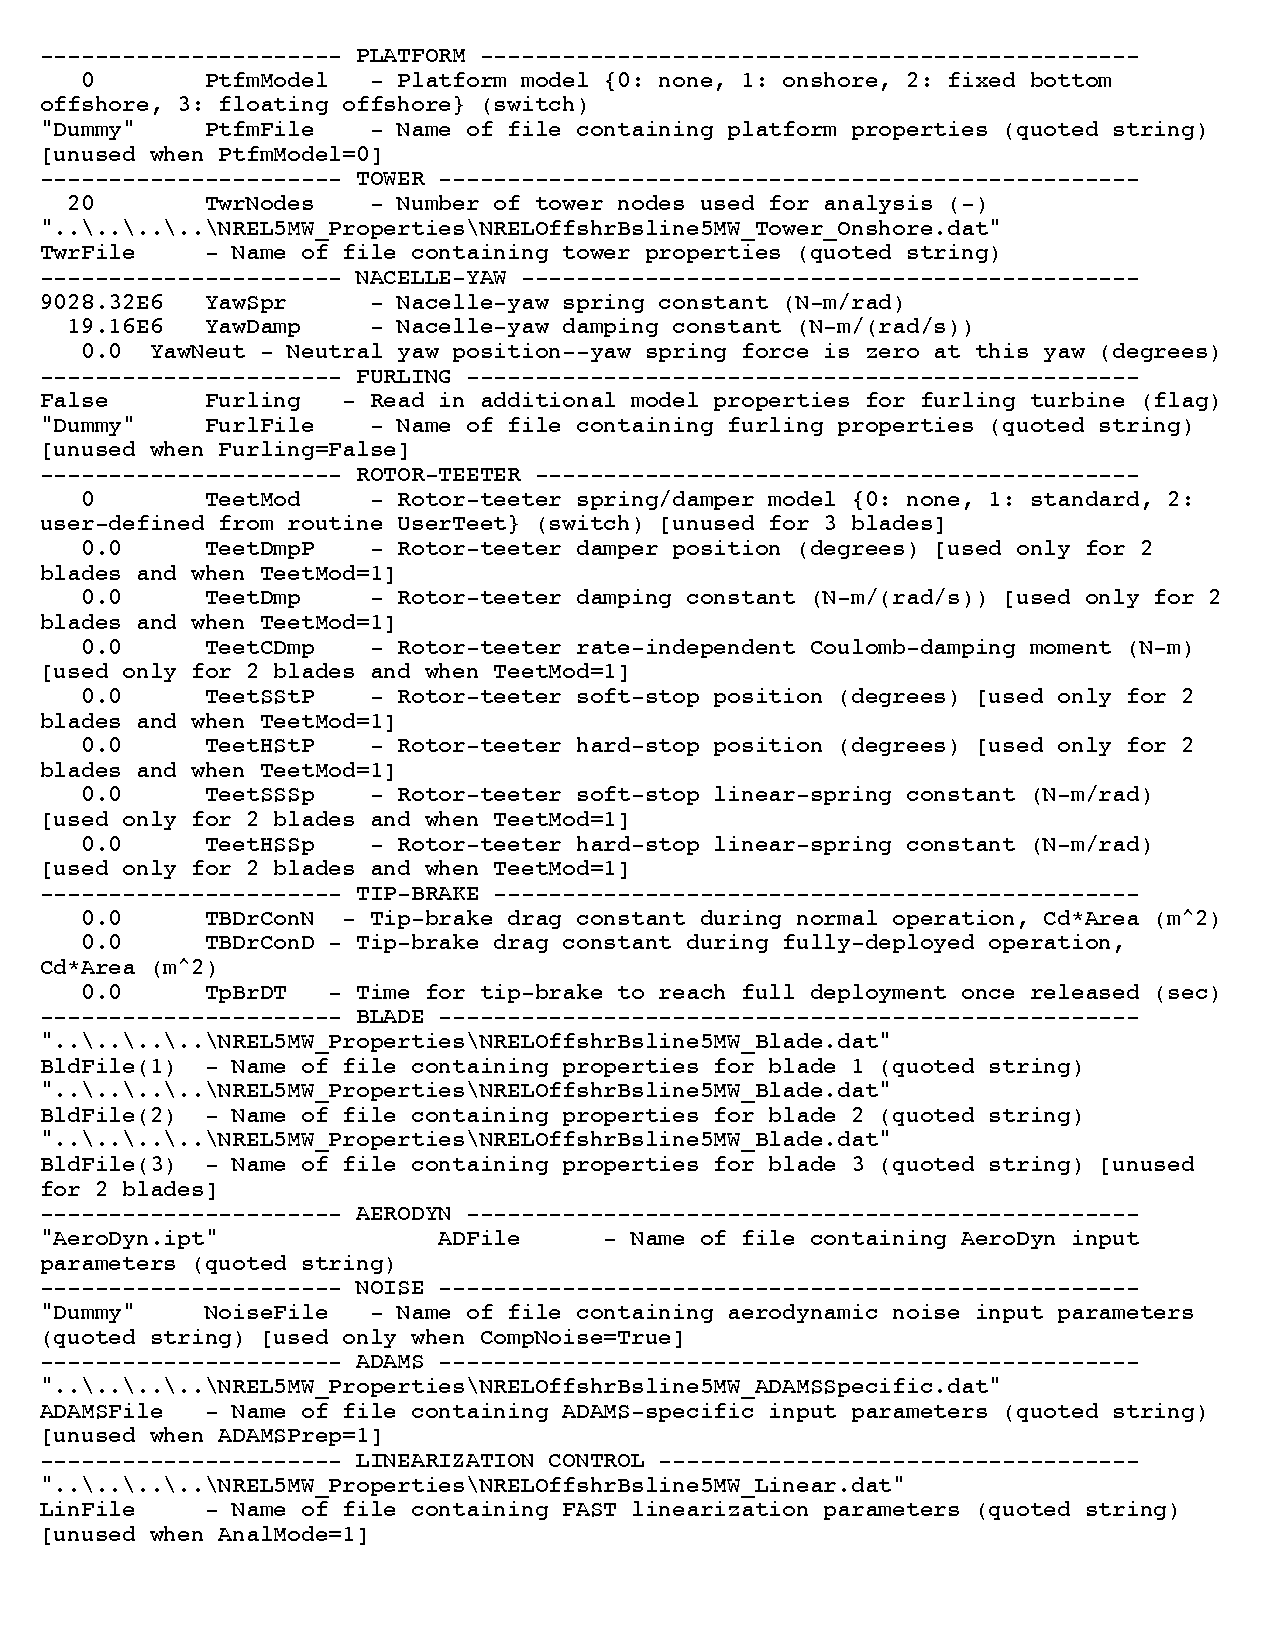
\includegraphics[width=\linewidth]{Figures/AppendixAFigures/primaryP4.pdf}	

\noindent
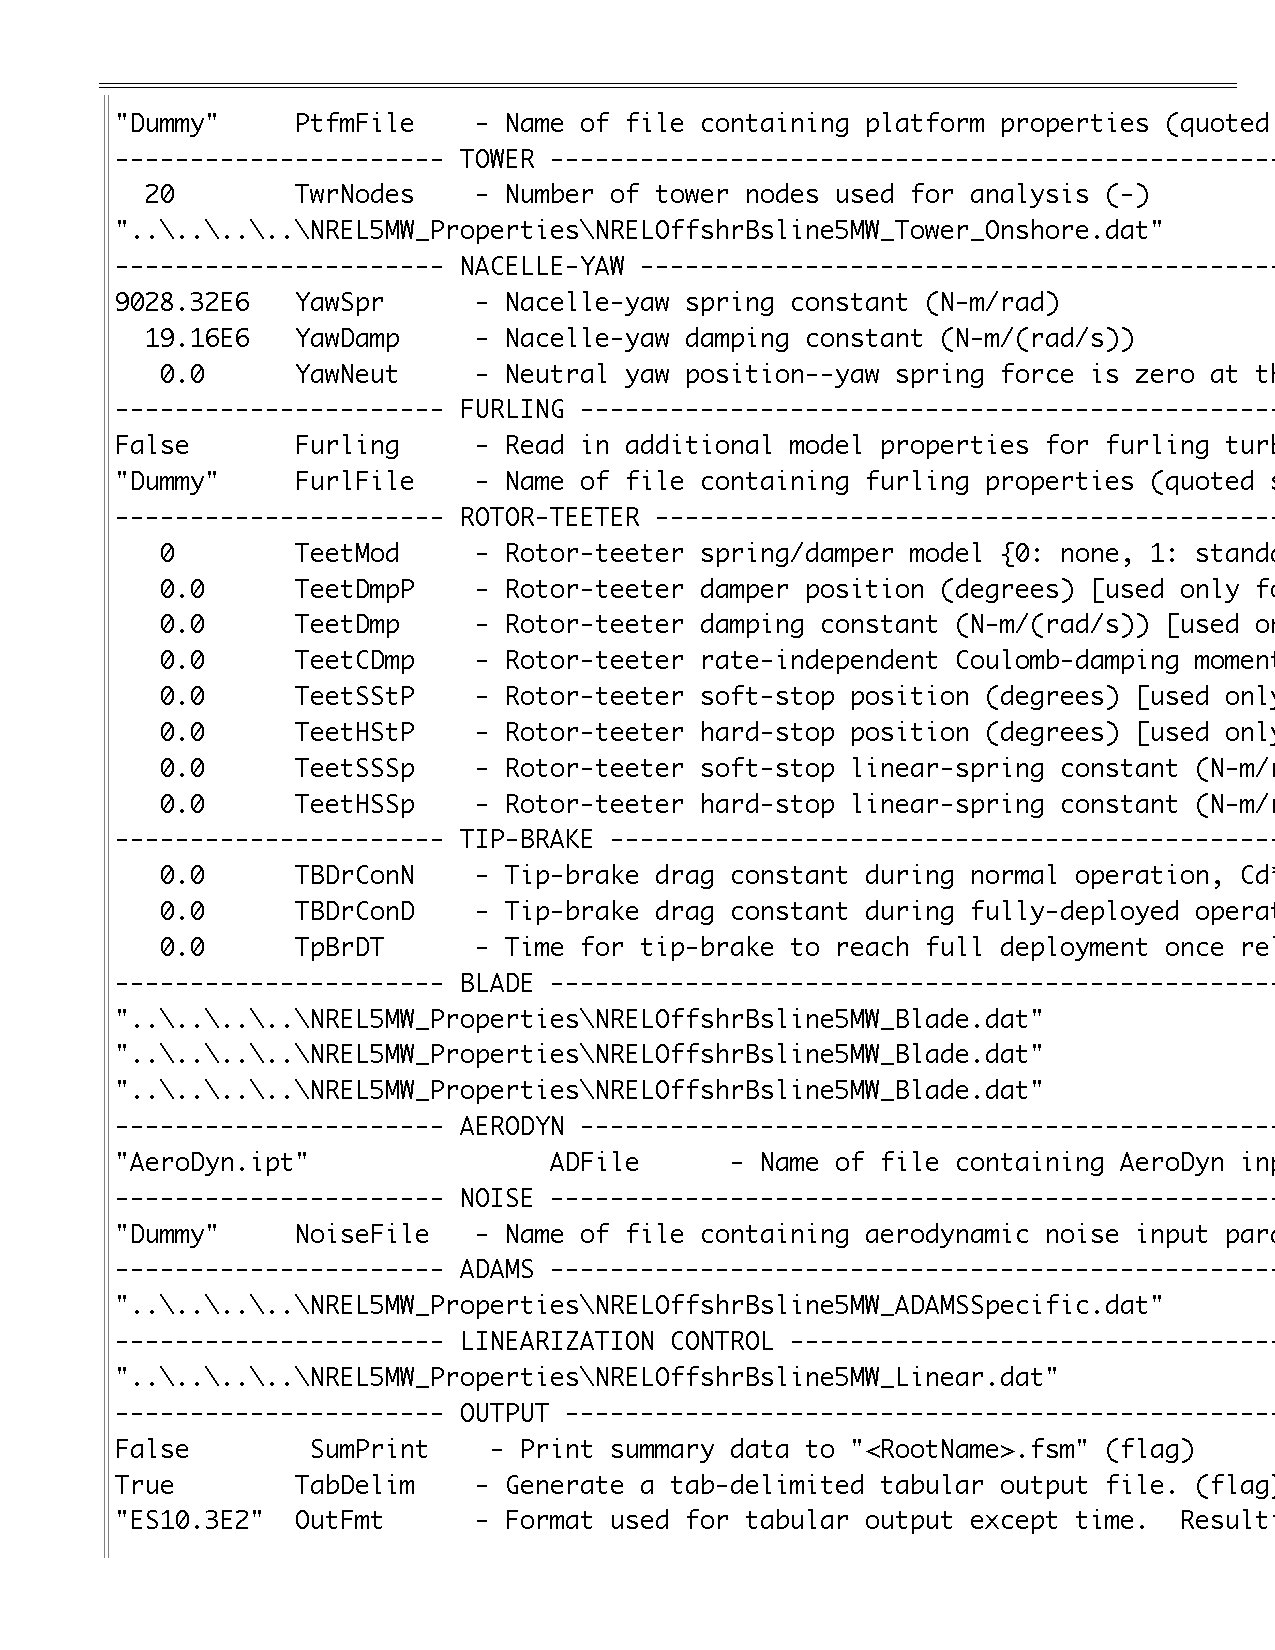
\includegraphics[width=\linewidth]{Figures/AppendixAFigures/primaryP5.pdf}	



\section{Aerodyn.ipt} \label{sectionA-2}

\noindent
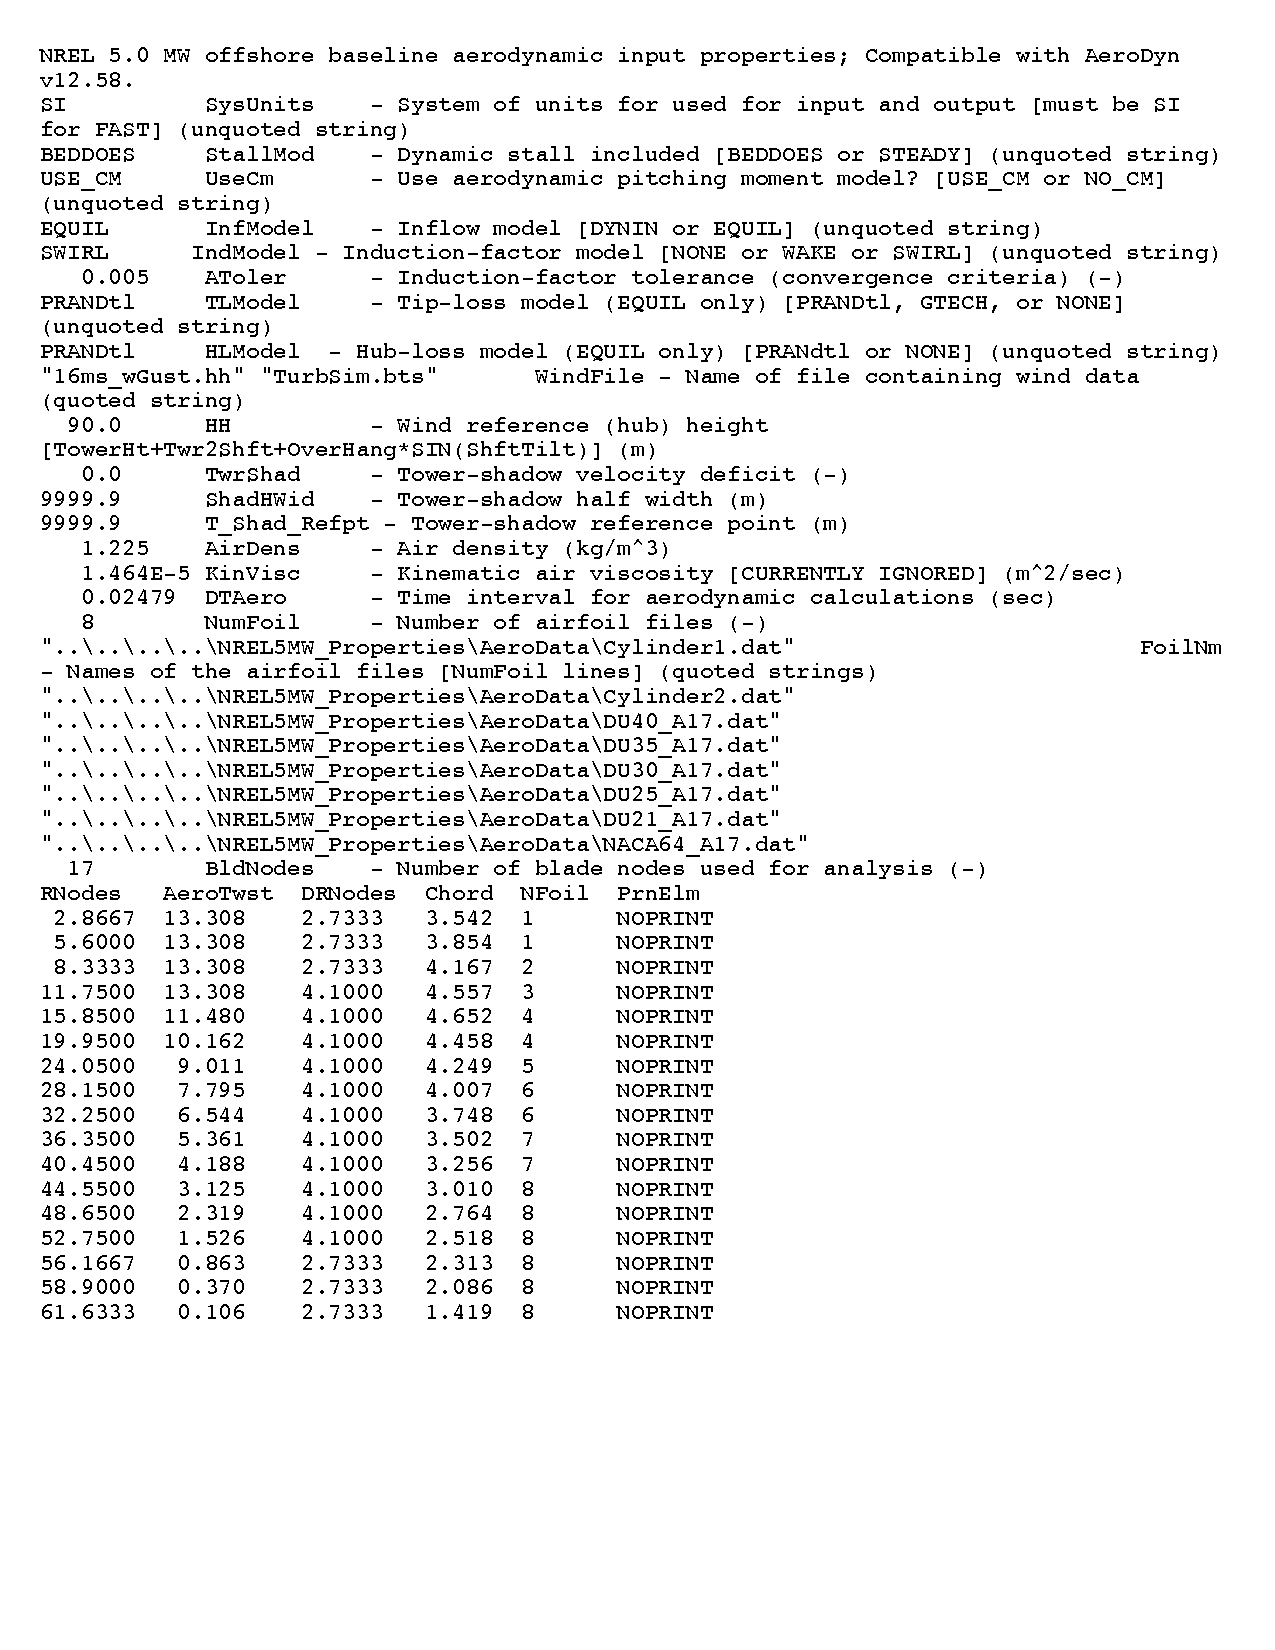
\includegraphics[width=\linewidth]{Figures/AppendixAFigures/aerodyn.pdf}		
